\section{Progettazione}\label{sec:project}

% Devono essere esposte le scelte progettuali operate nelle varie fasi di sviluppo dell'elaborato.

% In questa sezione devono essere documentati gli schemi di progetto relativamente all'architettura complessiva del sistema e alle sue componenti di rilievo.
% Per le componenti software si può ricorrere ad esempio a diagrammi delle classi, di sequenza, stato, attività.
% Per le componenti hardware è possibile includere opportuni schemi in grado di descrivere l'architettura fisica adottata.

% Vincoli circa la lunghezza della sezione (escluse didascalie, tabelle, testo nelle immagini, schemi):
% Numero minimo di battute per 2 componenti: 12000
% Numero massimo di battute per 2 componenti: 21000

In questa \nameCref{sec:project} viene presentata l'architettura generale del sistema,
partendo da come è stata derivata a partire dai requisiti raccolti, seguendo un approccio top-down:
si affronterà quindi prima la progettazione dell'architettura ad alto livello
e in un secondo momento le effettive implementazioni e architetture di dettaglio.

Il primo passo compiuto è stata la stesura del diagramma dei casi d'uso, riportato in \Vref{fig:use-cases},
fondamentale per inquadrare correttamente le funzionalità da realizzare sulla base dei requisiti;
successivamente si è passati alla progettazione di ciascun elemento dell'architettura.

\subsection{Architettura generale del sistema}

Come detto, il punto di partenza per l'ideazione dell'architettura sono stati i casi d'uso e i requisiti non funzionali individuati in fase di analisi:
da questi ultimi emergeva infatti la necessità di creare un sistema distribuito, scalabile e allo stesso tempo di semplice accesso.

Fin da subito, è apparsa evidente l'esigenza di implementare un'architettura che potesse distinguere livello principali:

\begin{enumerate}
  \item
    un primo livello dovrebbe essere quello dei \emph{sensori IoT}, diffusi nell'ambiente (ad esempio, almeno uno per stanza);
    essi dovrebbero svolgere al massimo una minima elaborazione locale,
    in quanto appoggiarsi al livello successivo, computazionalmente più potente, permetterebbe una maggiore flessibilità sull'analisi dei dati raccolti.
  \item
    un secondo livello dovrebbe essere un qualche tipo di \emph{appliance in rete locale} (ad esempio, almeno uno per struttura),
    in grado di svolgere il ruolo di raccolta dei dati e di \emph{gateway} verso l'esterno;
  \item
    un terzo livello, più esterno, che svolge un ruolo di aggregazione ulteriore, oltre a fornire l'accesso ai dati delle strutture da reti differenti.
\end{enumerate}

Quella che siamo andati a delineare è dunque un'architettura molto simile al concetto di \textbf{Fog Computing} come descritto da Cisco~\cite{CiscoSystems2016} nella teorizzazione originale.

Definita dunque questa architettura di massima, si è delineato le entità principali del sistema:

\begin{description}
  \item[Sensori IoT]
    Il primo livello citato sopra è costituito da sensori in grado di collegarsi autonomamente col gateway tramite protocollo wireless (ad esempio, WiFi 2.4GHz).
    Nel prototipo che si intende realizzare, si intende monitorare una singola stanza e verrà utilizzato un singolo sensore;
    l'ambiente di studio, infatti, ha stanze di media grandezza, che vengono coperte ``di misura'' dalle antenne embedded nel PCB di molti sensori dotati di modulo WiFi.
  \item[Server Fog] % TODO: ricorda di sostituire edge con fog ovunque
    Il secondo livello sarà realizzato tramite un PC a basso consumo (presumibilmente basato su SoC ARM) incaricato di ospitare:
    \begin{itemize}
      \item il codice di backend per svolgere il ruolo di \emph{gateway} tra i sensori e il cloud;
      \item un'interfaccia web in grado di mostrare informazioni sull'ambiente monitorato;
      \item gli eventuali server necessari all'infrastruttura per la comunicazioni dei sensori con il backend (come ad esempio un \emph{message bus} o un \emph{publish/subscribe broker}).
    \end{itemize}
  \item[Cloud]
    Il livello cloud sarà realizzato appoggiandosi a un provider in grado di offrire:
    \begin{itemize}
      \item
        un servizio PaaS per l'hosting del codice di backend,
        preferibilmente implementato nella medesima tecnologia scelta per il livello Fog, al fine di massimizzare il riuso del codice.
      \item
        un servizio PaaS per l'hosting del codice di frontend web in grado di mostrare informazioni su tutti gli edifici monitorati (nel prototipo, uno solo).
      \item
        un servizio di database gestito, possibilmente ottimizzato verso un elevato I/O\@;
        per il momento, l'essere relazionale o meno non è considerato rilevante.
    \end{itemize}
\end{description}

In \Cref{fig:architecture} è riassunto graficamente quanto descritto sopra, oltre alle interazioni che verranno analizzate nella \nameCref{subsec:interaction} successiva.

\begin{figure}[H]
  \centering
  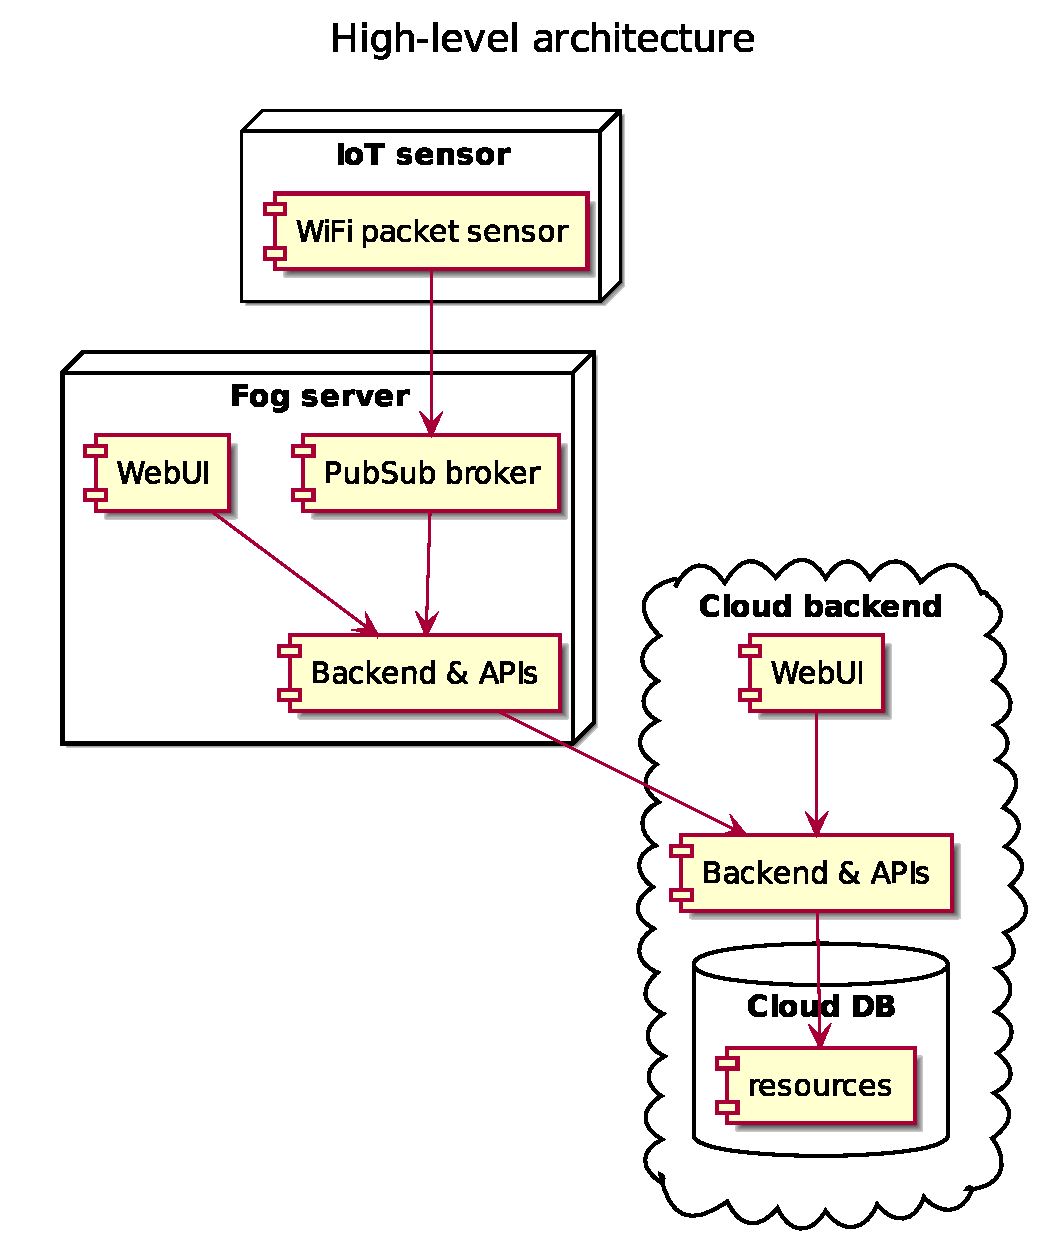
\includegraphics[width=0.7\textwidth]{res/out/architecture.eps}
  \caption{Componenti di massima dell'architettura e le loro interazioni}%
  \label{fig:architecture}
\end{figure}

\subsection{Interazioni tra gli elementi del sistema}\label{subsec:interaction}

Una volta individuate le entità fondamentali, il passo successivo è stato modellare le interazioni tra le componenti in gioco nel sistema.

Sulla base di quanto rappresentato nelle \Cref{fig:use-cases,fig:architecture}, sono stati analizzati i singoli scambi di informazioni tra le entità, analizzati come segue:

\begin{itemize}
  \item
    Per quanto riguarda la comunicazione tra il sensore e il Fog server, era necessario un protocollo di comunicazione leggero, veloce e non bloccante;
    per questi motivi, si è preferito un protocollo \emph{publish/subscribe} come MQTT~\cite{ISOCS2016}, che risulta perfetto per questi tipi di comunicazioni nell'ambito IoT.

    Per un corretto funzionamento, sarà necessario un \emph{MQTT broker} accessibile ad entrambi il Fog server e il sensore.
    Per quanto sia manualmente implementabile, si preferisce eseguire un software dedicato e indipendente;
    considerando eccessivo aggiungere un'altra macchina alla rete locale dedicata solo a questo scopo, il broker scelto verrà installato localmente al Fog server.

    In questo modo, il sensore può collegarsi al server tramite WiFi, sottoscriversi al broker come \emph{publisher}, pubblicare i dati raccolti e disconnettersi per riprendere il loop,
    mentre il backend, sottoscritto come \emph{subscriber}, si occupa di gestire quanto pubblicato.

    Si è scelto di esporre comunque API HTTP REST~\cite{Fielding2000}, che verranno utilizzate in modo asincrono dallo stesso Fog server e che permettono una espandibilità futura.
  \item
    Per quanto riguarda la comunicazione tra il Fog server e il backend in Cloud, si è ritenuto maggiormente indicato l'impiego di API REST\@.
    L'applicativo in esecuzione in cloud deve gestire le chiamate alle risorse, agendo sul database in modo asincrono e rispondendo di conseguenza.
  \item
    Per quanto riguarda le interfacce web, si è ritenuto ragionevole che il software di backend (sia Fog che Cloud) che gestisce le API possa anche servire tali pagine;
    esse, realizzate come \emph{Single Page Application}, sono in grado di risolvere le informazioni di cui hanno bisogno tramite chiamate HTTP alle API REST esposte dai rispettivi backend.
\end{itemize}

In \Cref{fig:measure} è riportato tramite diagramma UML di sequenza una rappresentazione con maggior dettaglio della procedura di registrazione di una misurazione.

\begin{figure}[H]
  \centering
  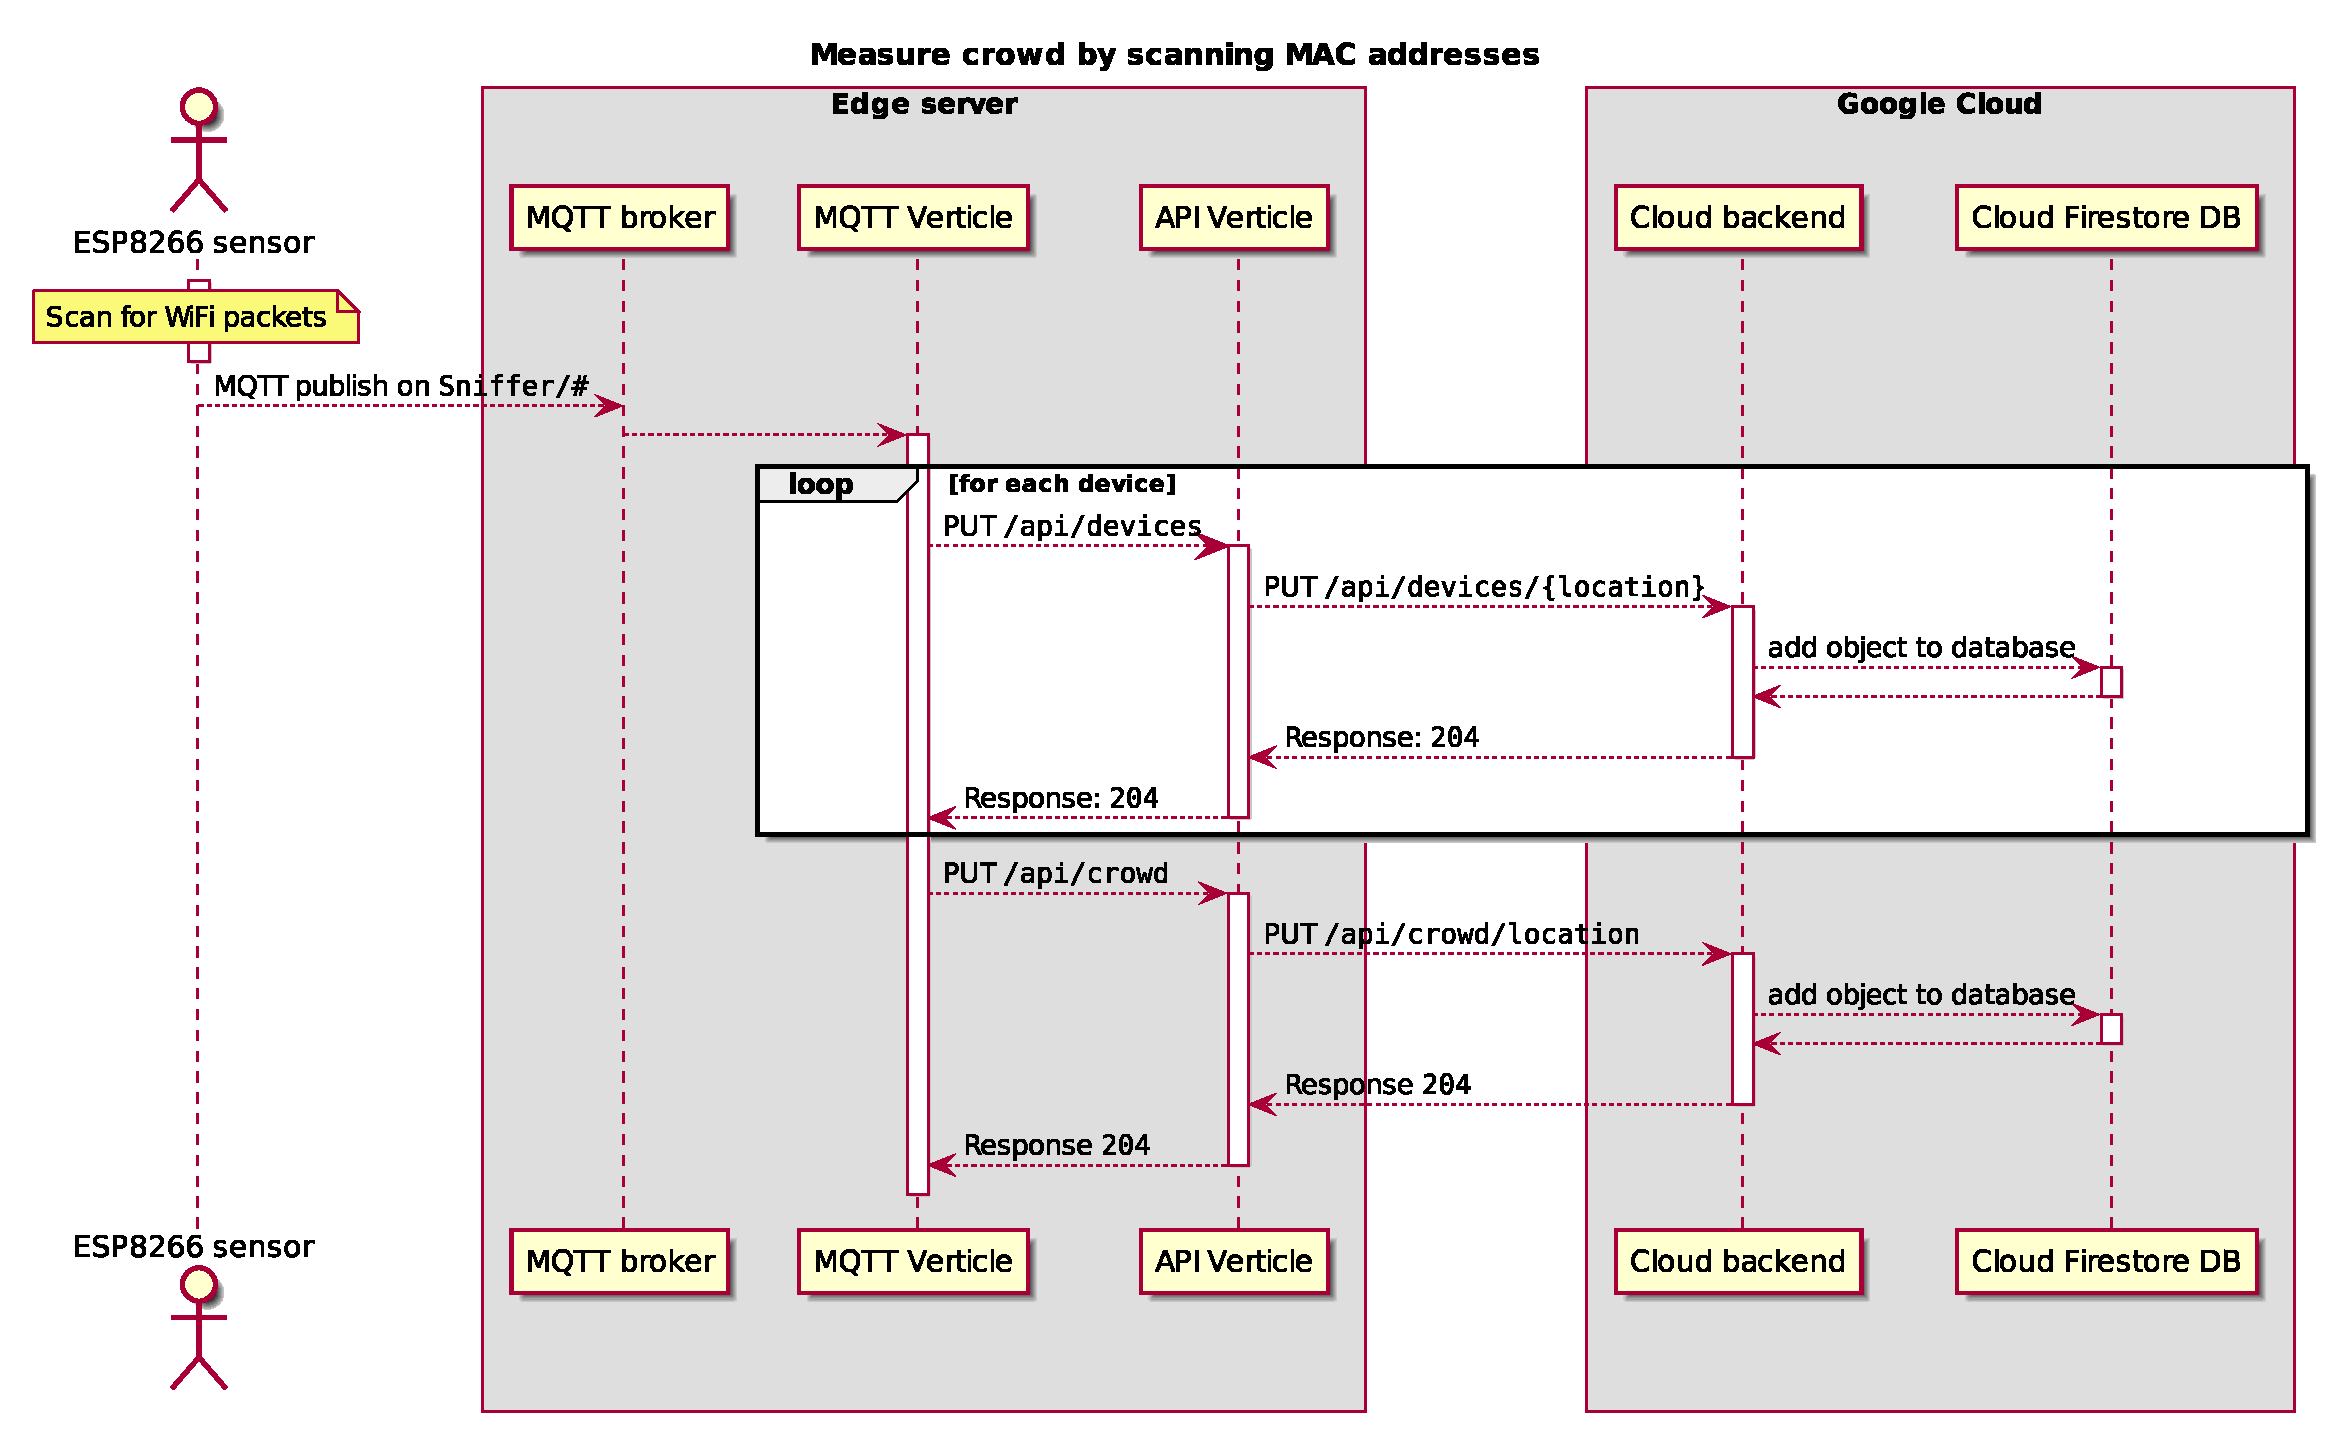
\includegraphics[width=\textwidth]{res/out/measure.eps}
  \caption{Diagramma UML di sequenza del processo di registrazione di una misurazione}%
  \label{fig:measure}
\end{figure}

\subsection{Cloud e Database}

Se nei passi di progettazione precedenti si è parlato solo genericamente di ``cloud'', è importante chiarire quale piattaforma è stata scelta:
infatti, differenti piattaforme possono offrire API che possono prestarsi o meno alle scelte architetturali anche di alto livello.
Nondimeno, per ottimizzare i costi conviene scegliere un database del medesimo provider, e anche in questo caso le differenze possono essere notevoli.

Tra i provider principali, la scelta è ricaduta sulla \strong{Google Cloud Platform}\footnote{\url{https://cloud.google.com/}}:
essa mette a disposizione un elevato numero di strumenti diversi, avendo quasi sempre il servizio adatto per il caso d'uso in questione.

Nel caso di questo progetto, l'ambiente di \strong{Google App Engine}, grazie al \emph{flex environment}, non pone limiti sull'architettura del codice in hosting, in quanto permette di appoggiarsi a immagini Docker\footnote{\url{https://www.docker.com/}} liberamente specificabili.

Spostando dunque l'attenzione alla componente database, la piattaforma mette a disposizione diverse scelte:
\emph{Cloud Spanner}, {Cloud SQL}, {Cloud Bigtable}, {Cloud Firestore}, {Firebase Realtime Database}, {Cloud Memorystore}.

Di questi, quelli che venivano proposti come adatti al dominio in questione sono i seguenti:

\begin{description}
  \item[Cloud SQL\footnotemark]\footnotetext{\url{https://cloud.google.com/sql}}
    Esso si pone come l'unica soluzione relazione tra quelli adottabili;
    offre tutte le proprietà tipiche dei DB SQL, ma richiede di appoggiarsi a un container \emph{Compute Engine} o \emph{Kubernetes Engine}, altre soluzioni a pagamento che si preferisce evitare per quanto possibile.
  \item[Firebase Realtime Database\footnotemark]\footnotetext{\url{https://firebase.google.com/products/realtime-database}}
    Esso è stato fino a poco tempo fa la soluzione ``standard'' per lo sviluppo di applicazioni Android tramite Firebase;
    il database (NoSQL documentale) è venduto come fortemente orientato al realtime e potrebbe essere indicato per gli utilizzi di questo progetto, ma l'SDK molto limitante al di fuori delle applicazioni mobile ce lo ha fatto evitare.
  \item[Cloud Firestore\footnotemark]\footnotetext{\url{https://cloud.google.com/firestore}}
    Esso è il database nato diversi anni dopo l'acquisizione di Firebase da parte di Google e vuole essere un ``upgrade'' del Firebase Realtime Database, dal quale eredita la natura NoSQL documentale e l'orientamento al realtime, ma ne migliora l'SDK e l'integrazione con le diverse piattaforme.
\end{description}

La soluzione scelta, come è possibile dedurre dall'elenco descrittivo sopra riportato, è il \strong{Cloud Firestore}.
Esso è in grado di garantire transazioni ACID mentre gestisce autonomamente i permessi di accesso, la replicazione e la notifica di \emph{osservatori} in realtime.

\subsection{Hardware necessario}

Per quanto riguarda le componenti hardware, come da requisiti il sistema non ha una complessità elevata.

Infatti, per rendere il sistema \emph{environment-aware} sono sufficienti i sensori WiFi (in questo prototipo, uno solo) disposti nell'ambiente.
Essi devono essere in grado di configurare il proprio modulo di ricezione WiFi in ``modalità promiscua'',
in modo da essere in grado di intercettare i pacchetti \emph{probe request} IEEE 802.11 inviati periodicamente dai dispositivi che tentano di riconnettersi a reti WiFi salvate.
Tali pacchetti contengono, tra le altre cose, l'SSID desiderato, il valore RSSI e l'indirizzo MAC \emph{in chiaro};
quest'ultimo è proprio l'oggetto di interesse della ricerca che deve essere intercettato.
Per un monitoraggio corretto, è necessario che tutti i canali previsti dal protocollo WiFi (e supportati dal sensore) vengano analizzati.

Essendo i sensori dotati di WiFi, non è necessaria una connessione differente per comunicare i dati,
bensì è sufficiente che il Fog server agisca da hotspot affinché il sensore vi si possa collegare per trasferire i dati raccolti ad ogni ciclo.
